\documentclass{beamer}

\usepackage{listings}
\lstset{
  columns=flexible,
  mathescape=true,
  keepspaces=true,
  showstringspaces=false,
  stringstyle=\slshape\color{green!40!black},
  basicstyle=\ttfamily\small,
  language=SQL,
  morekeywords={*, self},
  commentstyle=\slshape\color{black!60},
  tabsize=2,
}

\usetheme{metropolis}           % Use metropolis theme

\title{Optimizing Modern Data Processing Systems with Automated Reasoning}
\date{\today}
\author{Remy Wang}
\institute{University of Washington}
\begin{document}
  \maketitle

  \begin{frame}{Overview}
    \tableofcontents
  \end{frame}

  \section{Modern Data Processing}

  \begin{frame}{Modern Data Processing: Queries}
    Betweenness centrality of a graph $E$:
    \begin{align*}
      C(s, v) = \sum_{t: E(v, t) \wedge D(s, t)=D(s, v+1)} 
      \frac{\sigma(s, v)}{\sigma(s, t)}(1+ C(s, t))
    \end{align*}
    where $D$ is the distance, $\sigma$ is the \# of shortest paths. \pause
    \begin{itemize}
      \item Non-relational data \pause
      \item Aggregation \& interpreted functions \pause
      \item Recursive \pause
     \end{itemize}
    \textbf{Expressiveness} not well-supported by traditional optimizers:
    \[\#[R \times S] \Rightarrow \#[R] \cdot \#[S]\]
  \end{frame}

  \begin{frame}{Modern Data Processing: Data}
    \begin{columns}
      \begin{column}{{0.5\textwidth}}
        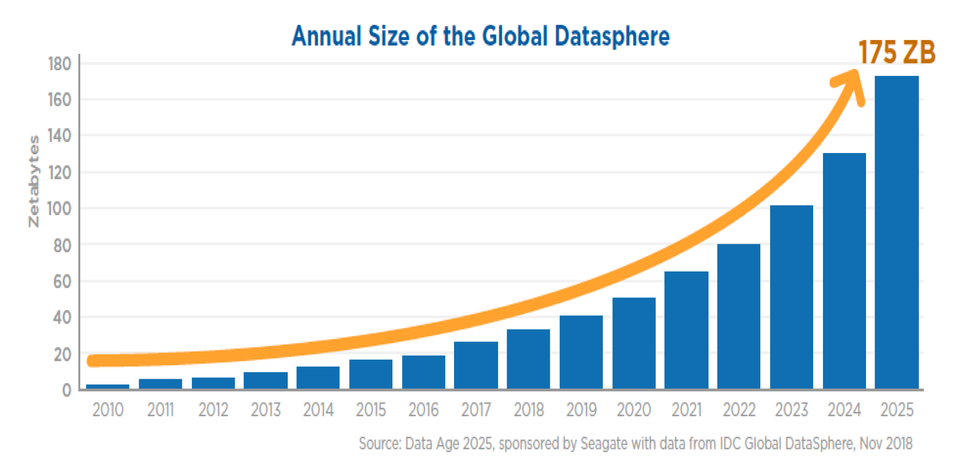
\includegraphics[width=\linewidth]{datasphere.png}
      \end{column}
      \begin{column}{{0.5\textwidth}}
        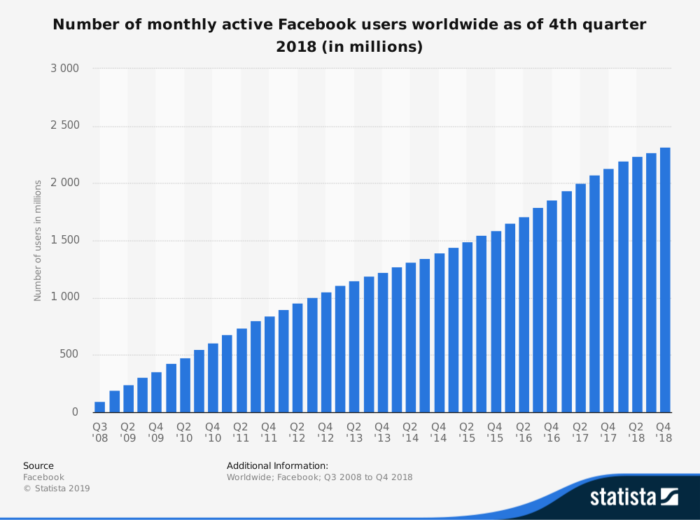
\includegraphics[width=\linewidth]{fb.png}
      \end{column}
    \end{columns}
    \begin{itemize}
      \item Data is increasing in \textbf{volume} \& \textbf{velocity} \pause
      \item The optimizer needs to produce faster plans in shorter time
    \end{itemize}
  \end{frame}

  \begin{frame}{Modern Data Processing: Systems}
    \begin{figure}
    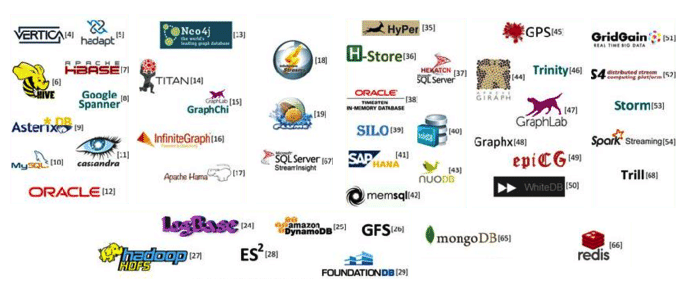
\includegraphics[width=\linewidth]{systems.png}
    \end{figure}
    \begin{itemize}
      \item Every data processing system needs an optimizer!
      \item Simplifying optimizers can save a lot of time for everyone.
    \end{itemize}
  \end{frame}

  \begin{frame}{My Theses}
    \begin{itemize}
      \item Core components and techniques from \textbf{automated reasoning}
      can make query optimizers simpler, more efficient,
      and more effective. \pause
      \item The \textbf{functional representation} of data can enable query 
      optimizers to effectively leverage automated reasoning tools.
    \end{itemize}
  \end{frame}

  \section{Background: Query Optimization and Reasoning}
  \section{The Functional Representation of Data}
  \section{Building Optimizers that Reason}
  \section{Proposal: Improving Optimizers with Reasoning}
\end{document}
